\documentclass{beamer}

\usepackage[utf8]{inputenc}
\usepackage[greek,english]{babel}
\usepackage{alphabeta}
\usepackage{amsmath}
\usepackage{graphicx}
\usepackage{hyperref}
\usepackage{xcolor}
\usepackage[dvipsnames]{xcolor}

\hypersetup{colorlinks=true, linkcolor=black, urlcolor=black, citecolor=black}

\title{HomeSense: Συλλογή και Οπτικοποίηση Περιβαλλοντικών Δεδομένων με Raspberry Pi}
\author{Ιορδάνης Κωστελίδης}
\date{03/02/2025}
\institute{Πρόγραμμα Μεταπτυχιακών Σπουδών στη Ρομποτική \\
Τμήμα Μηχανικών Πληροφορικής, Υπολογιστών και Τηλεπικοινωνιών \\
Σχολή Μηχανικών \\
Διεθνές Πανεπιστήμιο της Ελλάδος}

\begin{document}

\begin{frame}
\titlepage
\end{frame}

\begin{frame}
\frametitle{Εισαγωγή}
Το \textbf{HomeSense} είναι ένα ολοκληρωμένο σύστημα συλλογής και οπτικοποίησης περιβαλλοντικών δεδομένων που βασίζεται στο \textbf{Raspberry Pi 3B+} και σε τρεις ειδικά σχεδιασμένες συσκευές (GasSense, LightSense, TempSense).
\end{frame}

\begin{frame}
\frametitle{Αρχική Σελίδα}
	\centerline{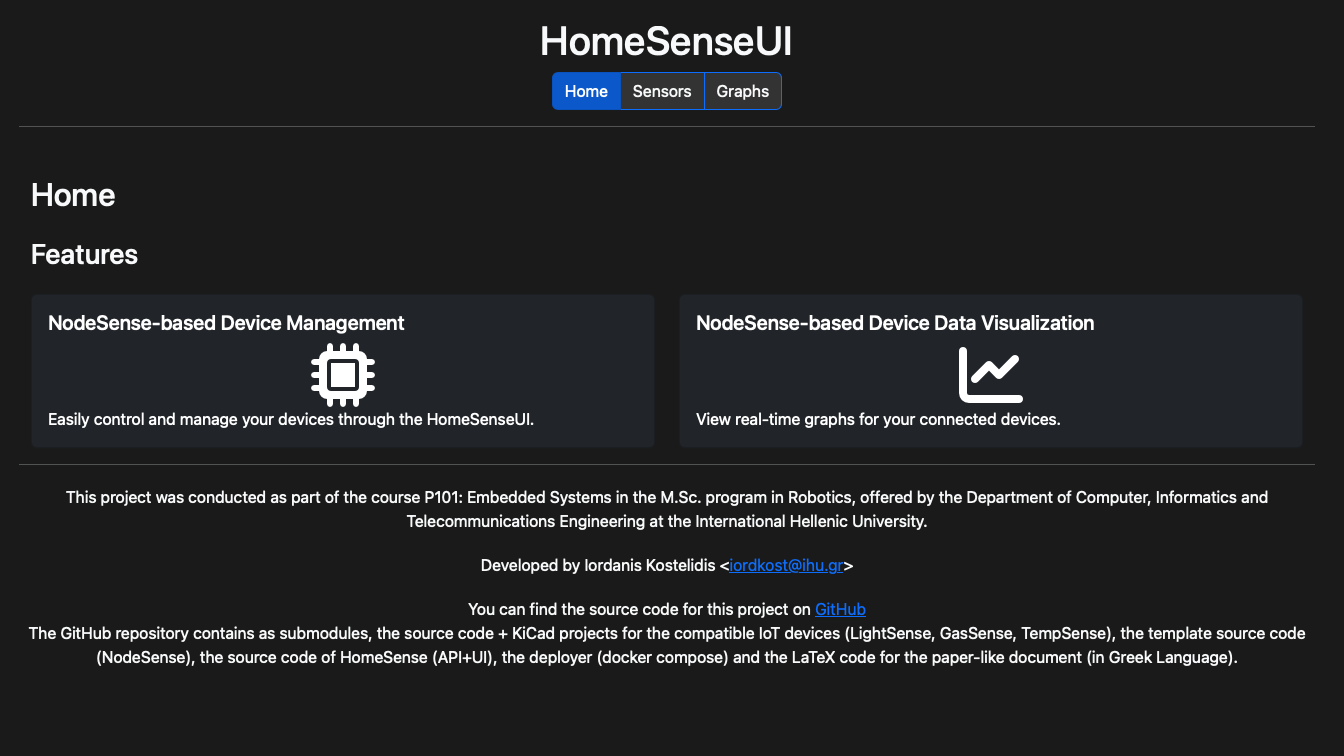
\includegraphics[width=1\textwidth]{assets/index-html}}
\end{frame}

\begin{frame}
\frametitle{Διαχείριση Αισθητήρων}
	\centerline{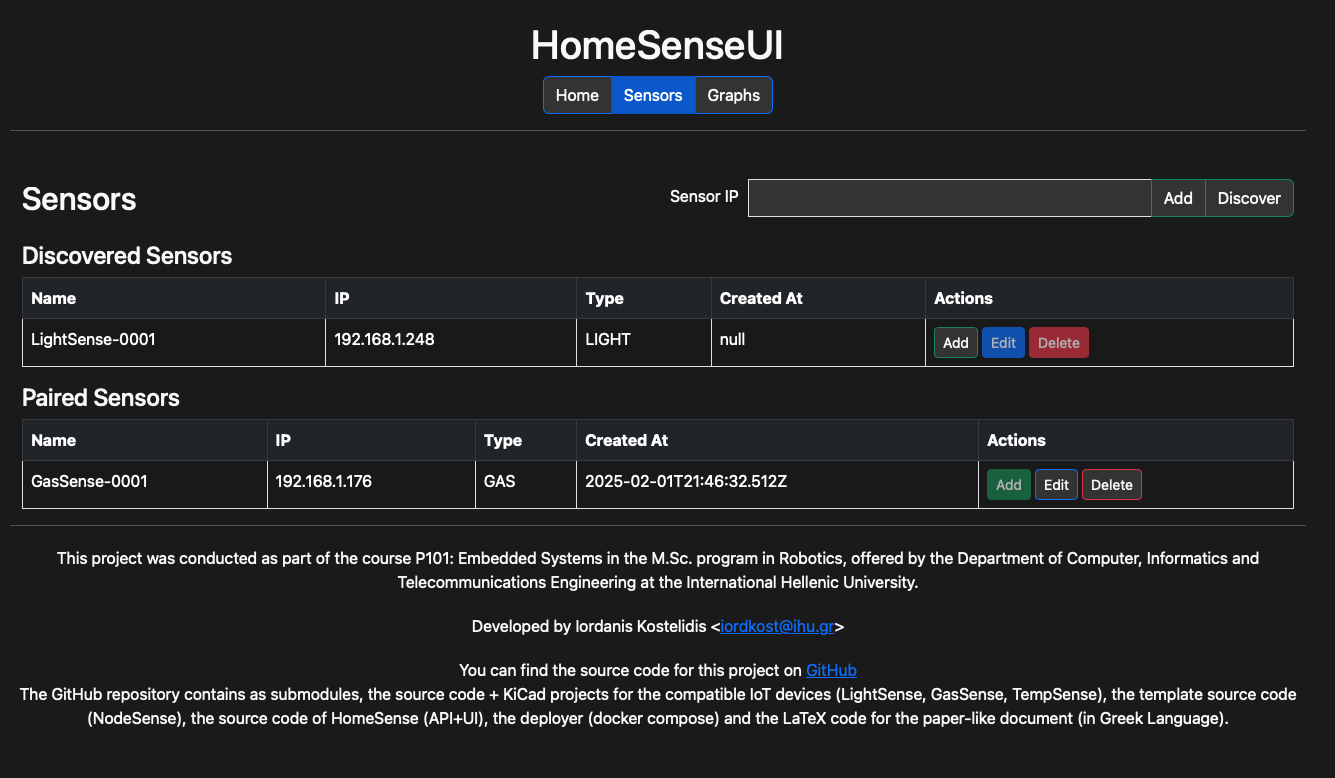
\includegraphics[width=1\textwidth]{assets/sensors-html}}
\end{frame}

\begin{frame}
\frametitle{Γραφήματα}
	\centerline{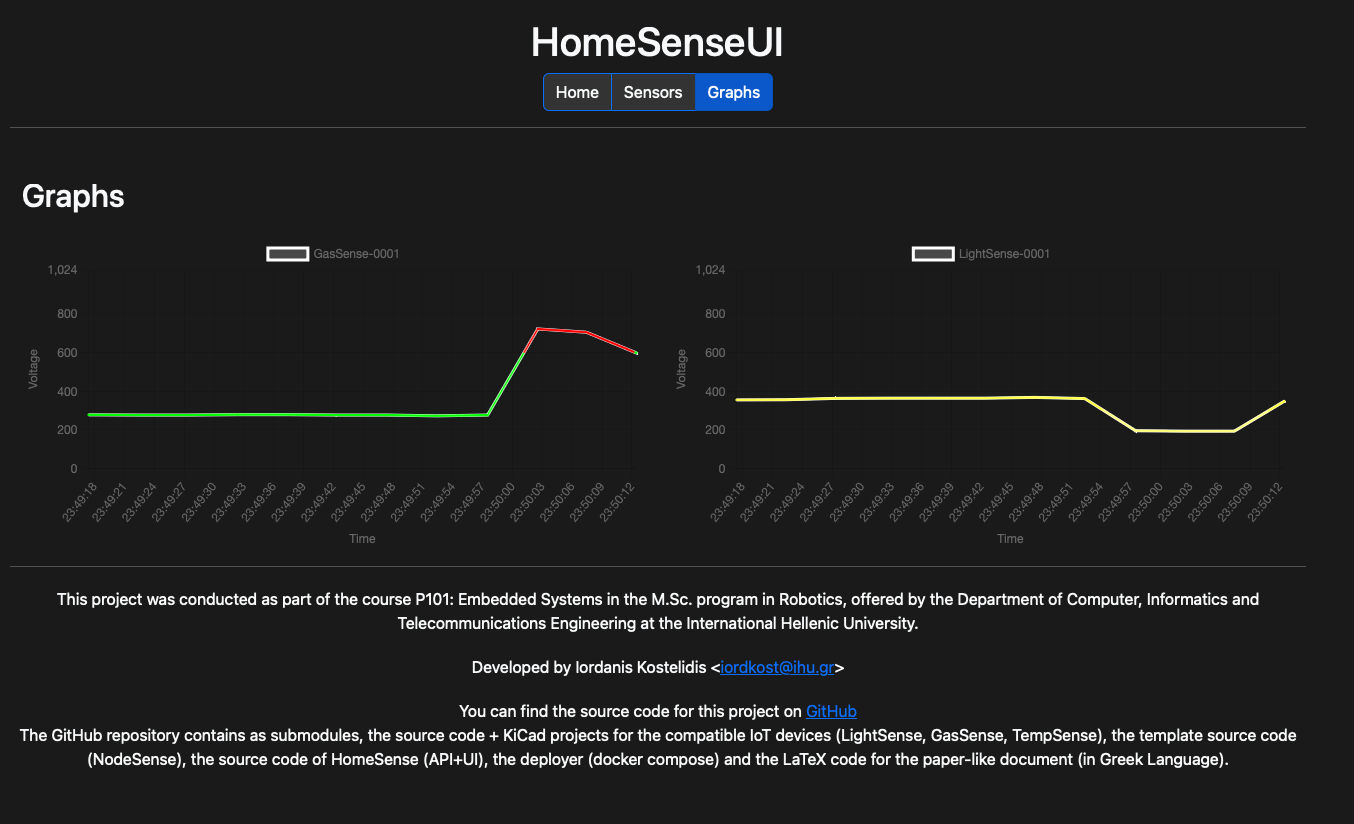
\includegraphics[width=1\textwidth]{assets/graphs-html}}
\end{frame}

\begin{frame}
\frametitle{Αρχιτεκτονική Συστήματος}
\begin{itemize}
    \item \textbf{Raspberry Pi 3B+}: Κεντρικός υπολογιστής του συστήματος για επεξεργασία και αποθήκευση δεδομένων.
    \item \textbf{NodeMCU ESP8266-based Devices}: Τρεις συσκευές που συνδέουν τους αισθητήρες στο δίκτυο Wi-Fi και κάνουν τα δεδομένα διαθέσιμα μέσω HTTP APIs. Οι αισθητήρες περιλαμβάνουν:
    \begin{itemize}
        \item \textbf{GasSense}: MQ-6 (αναλογικός) για την μέτρηση αερίων.
        \item \textbf{LightSense}: LDR (αναλογικός) για τη μέτρηση φωτεινότητας.
        \item \textbf{TempSense}: DS18B20 (ψηφιακός) για την μέτρηση θερμοκρασίας.
    \end{itemize}
\end{itemize}
\end{frame}

\begin{frame}
\frametitle{Σκοπός του Έργου}
Ο σκοπός του HomeSense είναι:
\begin{itemize}
    \item Η ασύρματη διασύνδεση μικροελεγκτών με ένα Raspberry Pi 3B+ για την καταγραφή και παρουσίαση δεδομένων από τρεις αισθητήρες  
\end{itemize}
\end{frame}

\begin{frame}
\frametitle{Raspberry Pi 3B+}
Το Raspberry Pi 3B+ είναι ο κεντρικός κόμβος του συστήματος, υπεύθυνος για:
\begin{itemize}
    \item Εκτέλεση εφαρμογών για την ληψη των δεδομένων.
    \item Διαχείριση της βάσης δεδομένων για αποθήκευση των ιστορικών δεδομένων.
    \item Παροχή διαδικτυακής διεπαφής για την οπτικοποίηση των δεδομένων.
\end{itemize}
\end{frame}

\begin{frame}
\frametitle{NodeMCU ESP8266-based Devices}
Οι συσκευές (GasSense, LigthSense, TempSensge) ειναι βασισμένες στο λογισμικό NodeSense το οποίο είναι συμβατό με τον μικροελεγκτή NodeMCU (ESP8266):
\begin{itemize}
    \item Είναι μικρό σε μέγεθος και έχει χαμηλή κατανάλωση ενέργειας.
    \item Έχει εύκολη ενσωμάτωση με το Raspberry Pi (μέσω HTTP API).
    \item Προγραμματίζετε εύκολα με το Arduino IDE, αλλά και με άλλες πλατφόρμες (π.χ. CLion with PlatformIO)
\end{itemize}
\end{frame}

\begin{frame}
\frametitle{GasSense Schematic}
	\centerline{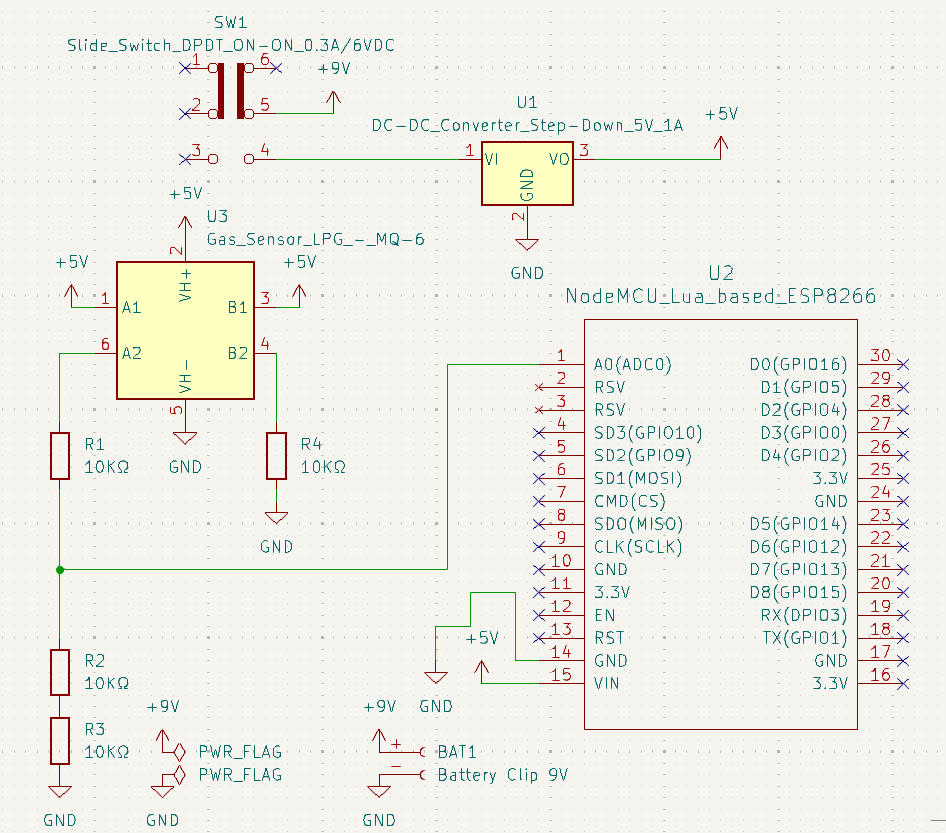
\includegraphics[height=0.6\textwidth]{assets/gassense-schematic}}
\end{frame}
\begin{frame}
\frametitle{GasSense PCB}
	\colorbox{PineGreen}{\centerline{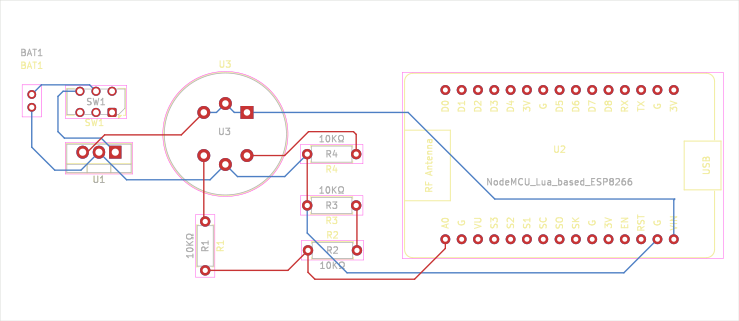
\includegraphics[height=0.4\textwidth]{assets/GasSense-brd}}}
\end{frame}

\begin{frame}
\frametitle{LightSense Schematic}
	\centerline{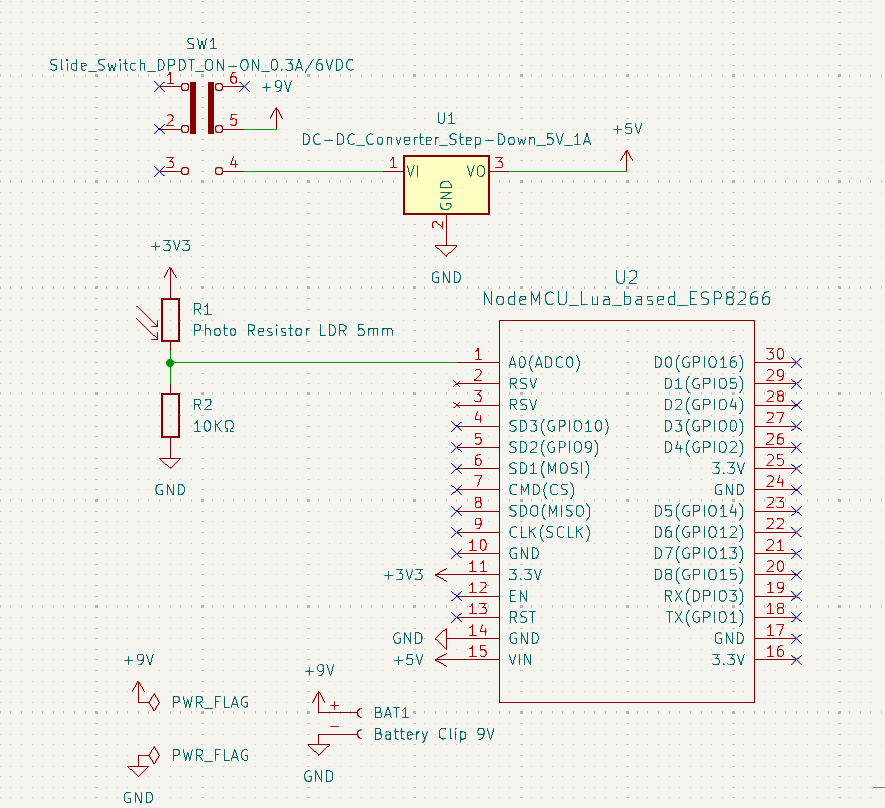
\includegraphics[height=0.6\textwidth]{assets/lightsense-schematic}}
\end{frame}
\begin{frame}
\frametitle{LightSense PCB}
	\colorbox{PineGreen}{\centerline{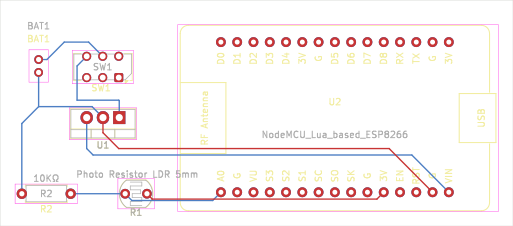
\includegraphics[height=0.4\textwidth]{assets/LightSense-brd}}}
\end{frame}

\begin{frame}
\frametitle{TempSense Schematic}
	\centerline{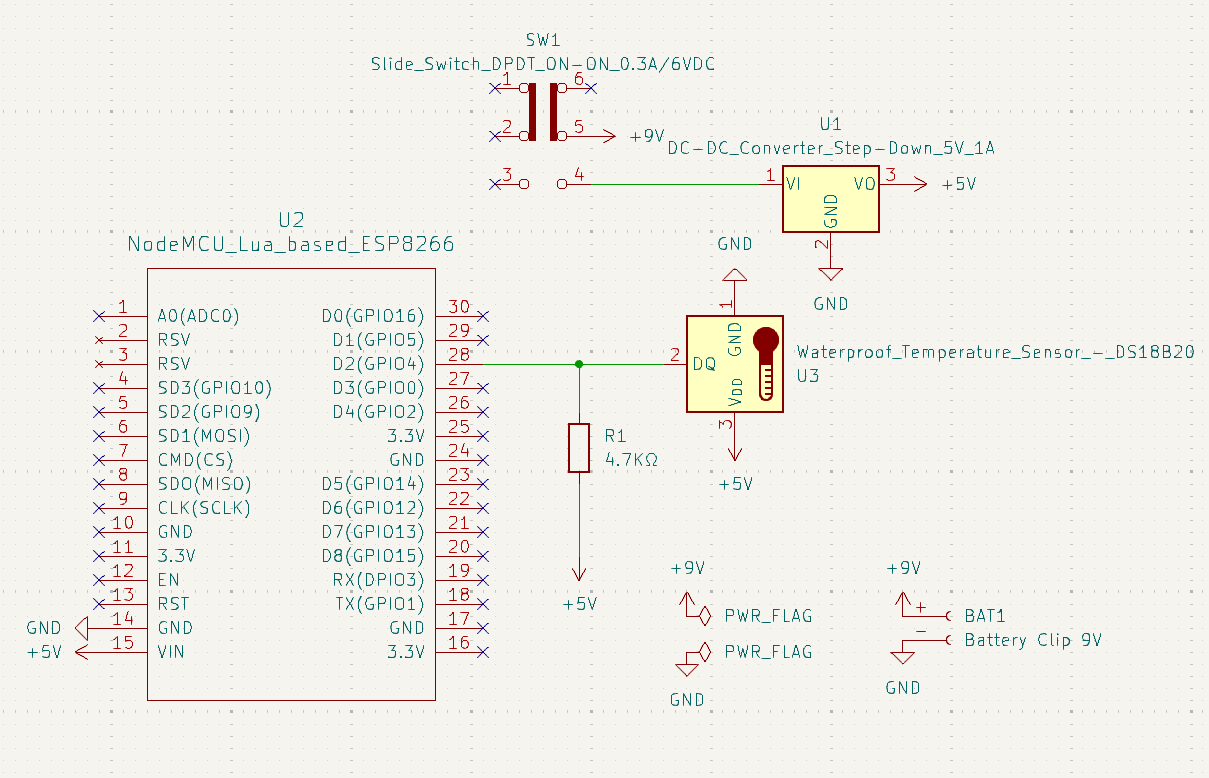
\includegraphics[height=0.6\textwidth]{assets/tempsense-schematic}}
\end{frame}
\begin{frame}
\frametitle{TempSense PCB}
	\colorbox{PineGreen}{\centerline{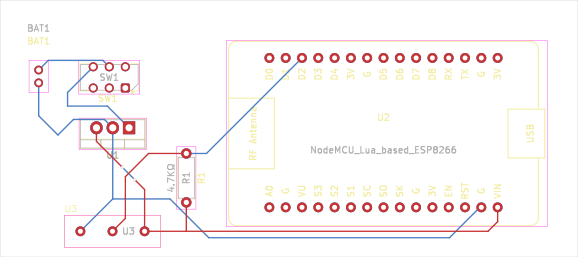
\includegraphics[height=0.4\textwidth]{assets/TempSense-brd}}}
\end{frame}

\begin{frame}
\frametitle{Διαδικασία Συλλογής Δεδομένων}
\begin{itemize}
    \item Ο χρήστης μέσω του UI κάνει pair τις συσκευές με το API.
    \item Το API, κάθε 5 δευτερόλεπτα, κάνει HTTP Call προς τη συσκευή για να λάβει τα δεδομένα του αισθητήρα.
    \item Το API, αναλύει τα δεδομένα και τα αποθηκεύει σε βάση δεδομένων PostgreSQL.
\end{itemize}
\end{frame}

\begin{frame}
\frametitle{Οπτικοποίηση Δεδομένων}
Τα δεδομένα οπτικοποιούνται μέσω μιας διαδικτυακής εφαρμογής που παρέχει:
\begin{itemize}
    \item Προσθαφαίρεση των συσκευών
    \item Γραφήματα σε πραγματικό χρόνο.
\end{itemize}
\end{frame}

\begin{frame}
\frametitle{It's Demo Time}
DEMO TIME
\end{frame}

\begin{frame}
\frametitle{Εργαλεία και Τεχνολογίες που Χρησιμοποιούνται}
\begin{itemize}
    \item \textbf{Docker}: Χρησιμοποιείται για την απομόνωση και εκτέλεση των εφαρμογών στο Raspberry Pi 3B+ 
    \item \textbf{PostgreSQL}: Βάση δεδομένων για την αποθήκευση των δεδομένων των αισθητήρων.
    \item \textbf{Spring Boot}: Χρησιμοποιείται για την ανάπτυξη του API.
    \item \textbf{HTML/CSS/JavaScript}: Χρησιμοποιείται για την ανάπτυξη του UI.
    \item \textbf{KiCad}: Για την σχεδίαση των συσκευών (Schematic και PCB).
    \item \textbf{CLion with PlatformIO}: Για την ανάπτυξη του λογισμικού των συσκευών.
    \item \textbf{TexShop}: Για την συγγραφή του κειμένου και της παρουσίασης.
\end{itemize}
\end{frame}

\begin{frame}
\frametitle{Μελλοντική Ανάπτυξη}
\begin{itemize}
    \item Επέκταση του συστήματος για την υποστήριξη περισσότερων αισθητήρων.
    \item Ενσωμάτωση με άλλα συστήματα για πλήρη αυτοματοποίηση.
\end{itemize}
\end{frame}

\begin{frame}
\frametitle{Source Code}
\begin{quote}
Talk is cheap. Show me the code.  
\\ \hfill -- Linus Torvalds
\end{quote}
\end{frame}

\begin{frame}
\frametitle{Source Code}
\begin{quote}
Πόσα repository?
\begin{itemize}
    \item 
\end{itemize}
\end{quote}
\end{frame}

\begin{frame}
\frametitle{Source Code}
\begin{quote}
Πόσα repository?
\begin{itemize}
    \item \textbf{1}?
\end{itemize}
\end{quote}
\end{frame}

\begin{frame}
\frametitle{Source Code}
\begin{quote}
Πόσα repository?
\begin{itemize}
    \item \textbf{1}? ΟΧΙ
\end{itemize}
\end{quote}
\end{frame}

\begin{frame}
\frametitle{Source Code}
\begin{quote}
Πόσα repository?
\begin{itemize}
    \item \textbf{5}?
\end{itemize}
\end{quote}
\end{frame}

\begin{frame}
\frametitle{Source Code}
\begin{quote}
Πόσα repository?
\begin{itemize}
    \item \textbf{5}? ΟΧΙ
\end{itemize}
\end{quote}
\end{frame}

\begin{frame}
\frametitle{Source Code}
\begin{quote}
I don’t have a 'mono-repo' project. I have an ‘ten-repo’ project.
\\ \hfill -- ??? ???
\end{quote}
\end{frame}

\begin{frame}
\frametitle{Source Code}
\begin{quote}
I don’t have a 'mono-repo' project. I have an ‘ten-repo’ project.
\\ \hfill -- Iordanis Kostelidis
\end{quote}
\end{frame}

\begin{frame}
\frametitle{Source Code}
\begin{itemize}
	\item NodeSense: Το αποθετήριο το οποίο περιέχει τον template κώδικα των συσκευών το οποίο βρίσκεται στο \\
	\href{https://github.com/KostelidisDev/NodeSense}{github.com/KostelidisDev/NodeSense}
	\item KiCadGrobotronics: Το αποθετήριο το οποίο περιέχει, custom library για τα components που αγοράστηκαν, από το κατάστημα GRobotronics, το οποίο βρίσκεται στο \\
	\href{https://github.com/KostelidisDev/KiCadGrobotronics}{github.com/KostelidisDev/KiCadGrobotronics}
\end{itemize}
\end{frame}

\begin{frame}
\frametitle{Source Code}
\begin{itemize}
	\item TempSense: Το αποθετήριο το οποίο περιέχει τον κώδικα, το σχηματικό και το PCB της συσκευής με τον αισθητήρα θερμοκρασίας το οποίο βρίσκεται στο \\
	\href{https://github.com/KostelidisDev/TempSense}{github.com/KostelidisDev/TempSense}
	\item LightSense: Το αποθετήριο το οποίο περιέχει τον κώδικα, το σχηματικό και το PCB της συσκευής με τον αισθητήρα φωτός το οποίο βρίσκεται στο \\
	\href{https://github.com/KostelidisDev/LightSense}{github.com/KostelidisDev/LightSense}
	\item GasSense: Το αποθετήριο το οποίο περιέχει τον κώδικα, το σχηματικό και το PCB της συσκευής με τον αισθητήρα αερίου το οποίο βρίσκεται στο \\
	\href{https://github.com/KostelidisDev/GasSense}{github.com/KostelidisDev/GasSense}
\end{itemize}
\end{frame}

\begin{frame}
\frametitle{Source Code}
\begin{itemize}
	\item HomeSense: Το αποθετήριο το οποίο περιέχει τον κώδικα του API και του UI το οποίο βρίσκετε στο \\
	\href{https://github.com/KostelidisDev/HomeSense}{github.com/KostelidisDev/HomeSense}
	\item HomeSense Deployer: Το αποθετήριο το οποίο περιέχει τον deployer για το API και το UI μέσω Docker Compose το οποίο βρίσκεται στο \\
	\href{https://github.com/KostelidisDev/HomeSense-Deployer}{github.com/KostelidisDev/HomeSense-Deployer}
	\item HomeSense-Document: Το αποθετήριο το οποίο περιέχει τον LaTeX κώδικα της εργασίας το οποίο βρίσκεται στο \\
	\href{https://github.com/KostelidisDev/HomeSense-Document}{github.com/KostelidisDev/HomeSense-Document}
	\item HomeSense-Presentation: Το αποθετήριο το οποίο περιέχει τον LaTeX κώδικα της παρουσίασης το οποίο βρίσκεται στο \\
	\href{https://github.com/KostelidisDev/HomeSense-Presentation}{github.com/KostelidisDev/HomeSense-Presentation}
\end{itemize}
\end{frame}

\begin{frame}
\frametitle{Source Code}
\begin{itemize}
	\item HomeSense-Platform: Το κεντρικό αποθετήριο το οποίο έχει ως sub-modules όλα τα σχετικά έργα του HomeSense το οποίο βρίσκεται στο \\
	\href{https://github.com/KostelidisDev/HomeSense-Platform}{github.com/KostelidisDev/HomeSense-Platform}
\end{itemize}
\end{frame}

\begin{frame}
\frametitle{Συμπεράσματα}
Το HomeSense αποτελεί μια ολοκληρωμένη λύση για τη συλλογή και οπτικοποίηση περιβαλλοντικών δεδομένων. 
Με τη χρήση του Raspberry Pi, του NodeMCU και του Docker, προσφέρει ευελιξία, επεκτασιμότητα και αξιοπιστία.
\end{frame}

\begin{frame}
\frametitle{Ευχαριστίες}
Ευχαριστώ για την προσοχή σας. Είμαι διαθέσιμος για τυχόν ερωτήσεις!
\end{frame}

\end{document}